\subsection{Tunneleffekt}
Der Tunneleffekt, auf dem die Funktionsweise des RTM basiert, kann nichtrelativistisch mit der station�ren Schr�dingergleichung f�r Materiewellen beschrieben werden.
\begin{align}
E\psi = \hat{H}\psi
\end{align}
�ber das Korrespondenzprinzip erh�lt man aus dem klassischen nichtrelativistischen Hamiltonian f�r ein Teilchen im Potential $V$ die Ortsdarstellung der Schr�dingergleichung:
\begin{align}
E\psi = \left(\frac{-\hbar^2\Delta}{2m}+V\right)\psi
\end{align}
$|\psi|^2$ gibt dabei die Aufenthaltswarscheinlichkeit des Teilchens im Volumenelement $\text{d}V(\textbf{x})$ an. Der Tunneleffekt kann anhand eines einfachen Beispieles verstanden werden, indem in einer Dimension ein Potentialwall in Form eines Kastens angenommen wird. Ein veranschaulichendes Bild ist wichtiger, als ein langer Rechenweg, weshalb es vorzuziehen ist, die L�sung mit Abbildung \ref{fig:kastenpot_schroe} zu veranschaulichen.
\begin{figure}[H]
\centering
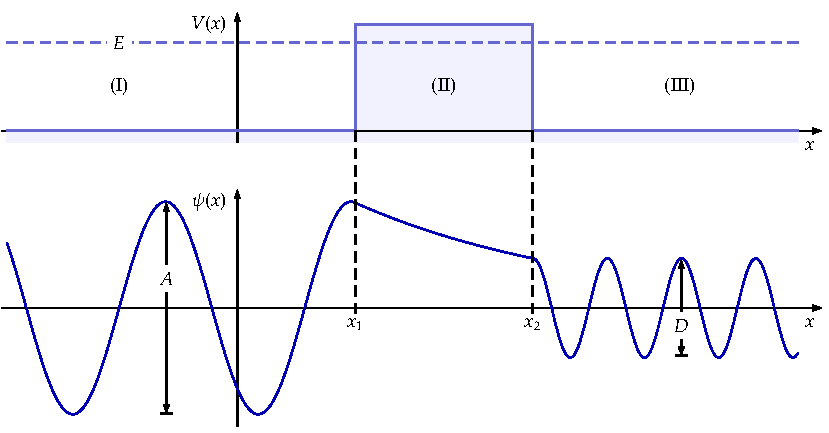
\includegraphics{tunneleffekt_wellenfunktion_und_potential_1}
\caption{Eindimensionale Schr�digergleichung mit Potentialwall in der Mitte. Zu sehen ist der exponentielle Abfall der Amplitude der Wellenfunktion, wodurch die Aufenthaltswarscheinlichkeit hinter dem Potentialwall $D^2$ kleiner als $A^2$ ist. (vgl. \cite{tunnel_pic})}
\label{fig:kastenpot_schroe}
\end{figure}
Der Rechenweg kann ohne Probleme auf der Seite \cite{wiki_tunnel} nachvollzogen werden. Die L�sung der Schr�dingergleichung innerhalb der Potentialbarriere ergibt einen exponentiellen Abfall der Aufenthaltswarscheinlichkeit mit zunehmender Eindringtiefe, wobei die Wellenl�nge gleich bleibt. Damit die Elektronen w�hrend des Versuches nicht in beide Richtungen gleich stark tunneln, wird eine Potentialdifferenz zwischen Bereich (I) und Bereich (III) erzeugt, woduch die Elektronen eine Vorzugsrichtung bekommen. Der Tunnelstrom $I_{Tunnel}$, die entscheidende Messgr��e, ist proportional zur Tunnelwarscheinlichkeit multipliziert mit der angelegten Spannung $V_{bias}$ und der Zustandsdichte $\rho_s$ bei der Fermienergie $E_f$:
\begin{align}
I_{Tunnel} \propto V_{bias}\rho_s(E_f)\exp[-2] \propto
\end{align}